\chapter{Gaussian Splatting for 360\degree spin stabilization}
\label{chapter:gausssplat}

\chapterwithfigures{\nameref*{chapter:gausssplat}} \chapterwithtables{\nameref*{chapter:gausssplat}}

\ifthenelse{\boolean{skipGauss}}{\endinput}{}

\section{Introduction}
This final section extends the latest two sections that were mostly focused toward a research academic perspective. Core motivation rather lies here on the desire to apply \ac{NVS} latest advances on an industrial project, where processed images resolution are at least $10\times$ higher than ShapeNet-SRN \citep{chang2015shapenet,sitzmann2019scene} ones ($\sim$ 1-2K against $128\times128$). \ac{NeRF} have benefited over the latest few years from massive improvements against several directions; training time, camera pose requirements, inference speed, drastic model weight reduction \textit{etc}. 
However, \ac{NeRF}-based methods suffers from an intrinsic computational bottleneck at inference time. It requires to query the \ac{NeRF} roughly 500 millions times to generate a squared $2K\times2K$ image. As a direct consequence, one of the most acknowledged state-of-the-art method, termed Mip-NeRF360 \citep{barron2022mip}, is only able to render at < 0.1 \ac{FPS} a 1080p image. It would therefore be necessary to deploy a lot of \ac{GPU} resources and engineering refactorization to properly parallelize the source code in order to synthesize novel views at acceptable speed. 

We thus work in this section with a different set of constraints. First concerns the generalizable property we kept in the two previous sections. We do not aim anymore to build or rely on an algorithm that can synthesize a viewpoint from any image belonging to a specific class. We thus rather want to leverage on \textit{per-scene} framework, that would require a novel training as soon as we work with a new scenario. Furthermore and as mentioned earlier, images we are now working with are closer to what clients could sent to any \ac{AI} SaS company, both regarding resolution and content. Finally, camera poses are no longer available as ground truth since real-world images CarCutter by Meero has to deal with are unposed. They thus must be first estimated using \ac{SFM} techniques (subsection \ref{subsec:gs-sfm}).

Core idea is rather to leverage on the very latest advances in neural rendering, mostly on \ac{GS} ones. \ac{GS} offers an extremely well balanced trade-off between rendering quality and training/inference requirements. Contrary to \ac{NeRF}-based methods, that are therefore often too slow to render high-resolution images, \ac{GS} shows an outrageously 100 \ac{FPS} performance, withtout relying on any neural network architecture. However, the \ac{NVS} paradigm we were used to deal with until now has heavely changed: View synthesis is not anymore infered given a source image and a camera transformation. As soon as \ac{GS} reconstructs the whole 3D scene through a set of 3D coloured gaussians, render a novel view now at a specific viewpoint only require a camera pose information.


\section{Background}
In order to be as close as possible to what was investigated for CarCutter and to remain consistent accross the experiments and tested methods, a single scene made of 36 views is used in this section. Figure \ref{fig:gs-original_scene} depicts such scene. This background section establishes fundamental concepts and algorithms that turn this unordered and unposed finite set of images into an explicit 3D scene that can be rendered from any viewpoint. 

\begin{figure*}[htb!]
    \center
  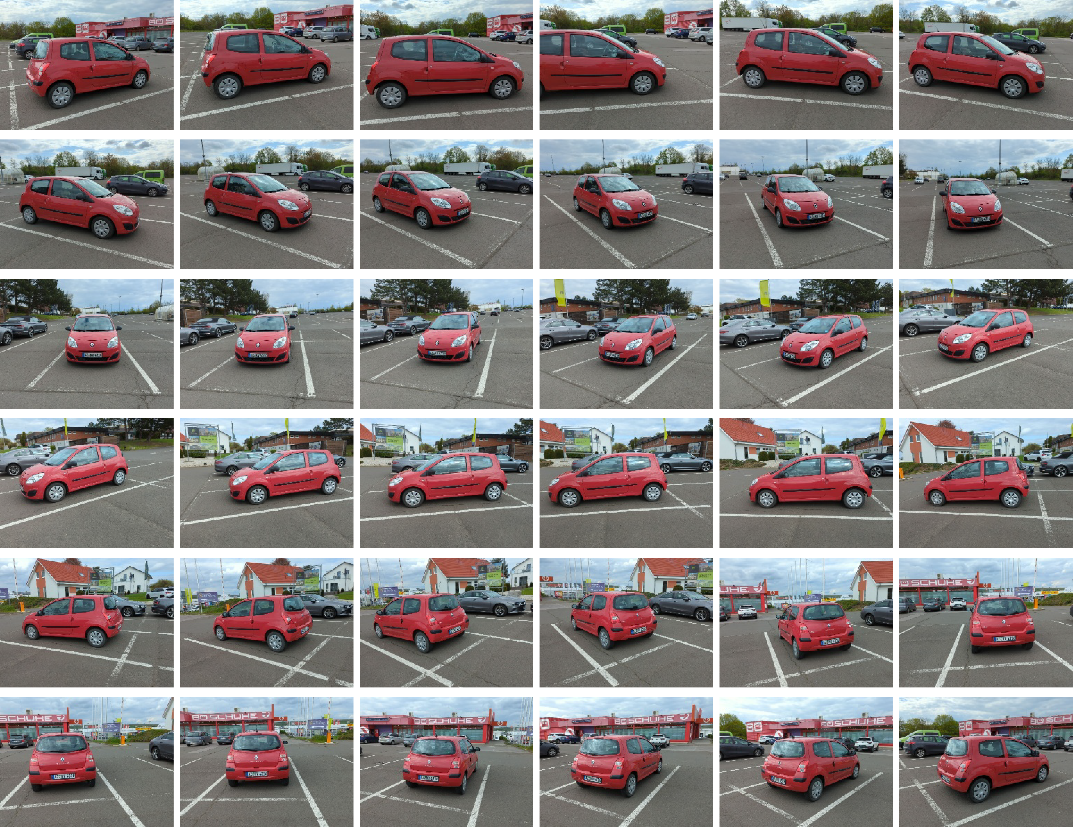
\includegraphics[height=10cm]{images/gaussiansplatting/original_scene.png}
  \caption{\textbf{Original scene.} Such a scene is typically what Carcutter is working with on a daily basis. A total of 36 unposed views has been acquired here. Distance from the car and camera viewpoint direction are not persistant across the different images.}
  \label{fig:gs-original_scene}
\end{figure*}

\subsection{Camera pose estimation through SfM with COLMAP}
\label{subsec:gs-sfm}

\begin{figure*}[htb!]
    \center
  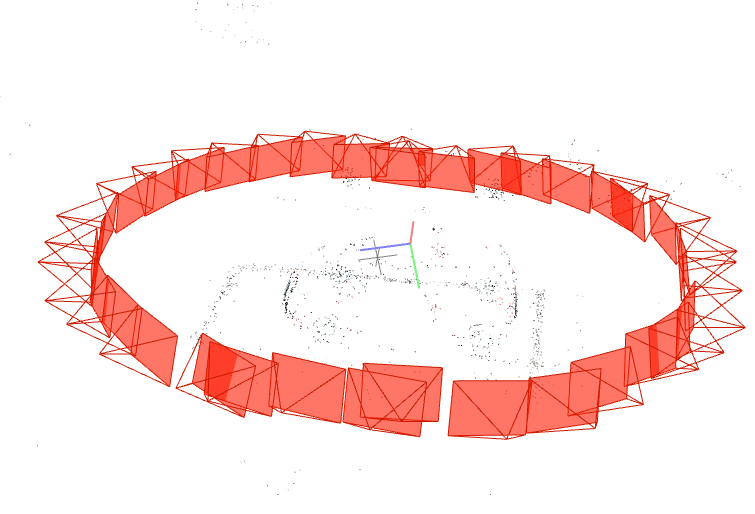
\includegraphics[height=8cm]{images/gaussiansplatting/colmap_sparsePC.png}
  \caption{\textbf{COLMAP 3D sparse reconstruction.} Given the set of unorded and unposed 36 views depicted below, COLMAP reconstructs an extremely sparse coloured point cloud with the corresponding estimated camera location. A total of $N=4105$ points has been registered here in this scenario.}
  \label{fig:gs-sfm}
\end{figure*}

\subsection{Gaussian Splatting}
\label{subsec:gs-sfm}

It exists a plaethora of different ways to represent 3D data, either explicitly (such as point clouds, meshes) or implicitly. \ac{NeRF} implicitly embeds the whole structure and texture of a scene in its inner weights: an image is rendered by sampling points on casted rays and quering the architecture accordingly. \ac{GS} rather leverages on a 3D gaussian primitive to explicitly model the 3D scene and get a fully differentiable pipeline that can solely be supervised at 2D-image level. Figure \ref{fig:gs-overview} gives few insights regarding how such a pipeline is built.  


\begin{figure*}[htb!]
    \center
  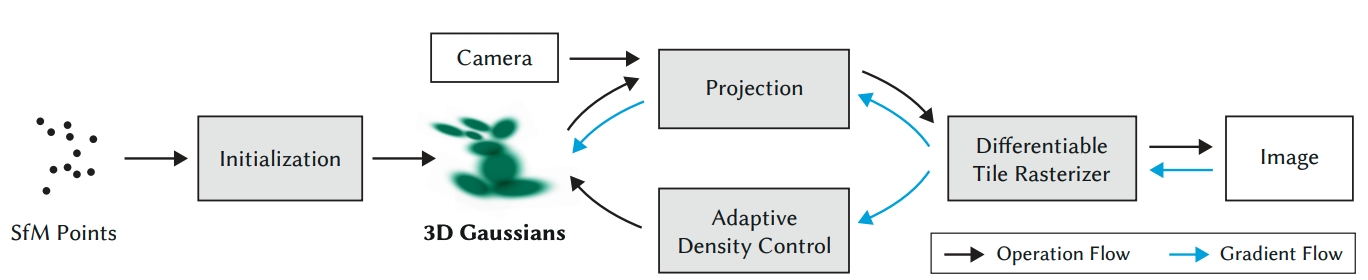
\includegraphics[height=6cm]{images/gaussiansplatting/overview-pipelineGS.png}
  \caption{\textbf{Gaussian Splatting pipeline overview.} Starting from a sparse 3D point cloud, \ac{GS} is designed on a lightweight and differentiable pipeline that does not involve any deep or shallow neural architectures.}
  \label{fig:gs-overview}
\end{figure*}


We present below the key steps that were defined in the original \ac{GS} seminal work \citep{kerbl20233d}.
\noindent \textbf{Initialization} From a sparse coloured \ac{SFM}-3D point cloud, refered as $M\in\mathbb{R}^{N\times(3+3)}$, an associated set of 3D Gaussians $\mathcal{G}$ is build. Each primitive $g \in \mathcal{G}$ has therefore an attached set of attributes $\{\mu,\Sigma,c,\alpha\}$, defined by: 
\begin{itemize}
    \item A mean $\mu$, corresponding to the original point location in $M$. 
    \item A covariance $\Sigma$ $3\times3$ matrix, that must be positive semi-definite. 
    \item A color $c$, represented using \ac{SH} coefficients. Additional information regarding \ac{SH} theory and construction can be found in the Appendix \label{appendix:gs-sh}. 
    \item An opacity/transparency $\alpha$ value. 
\end{itemize}
These attributes that are going to be learned, for all gaussians in  $\mathcal{G}$ during training. While mean, color and opacity can be optimized without any constraints with gradient-descent based algorithm, $\Sigma$ has to remain semi-definite positive \footnote{\textit{i.e} $ \forall a \in \mathbb{R}^{3}: a^{T}\Sigma a \geq 0$} during training to represent a meaningful 3D coviance matrix. As holding this constraint during the optimization would be to complex, $\Sigma$ is expressed in the world coordinate system via a reparametrization trick with a rotation $R$ (expressed as a quaternion during training in the source code) and a scaling matrix $S$: 

\begin{equation}
    \Sigma = RSS^{T}R^{T}
\end{equation}
As any matrix expressed by $A^{T}A$ is always semi-definite positive, $\Sigma$ is now properly constrained. Term $RS$ has to be seen as scaled rotation matrix, where $R$ defines the Gaussian rotation in space and $S$ its size.  

\noindent \textbf{3D Gaussian projection}
\noindent \textbf{Tile-based differentiable rasterizer}
\noindent \textbf{Densification and Pruning strategy}

\section{Related Work}
\section{Method}
\subsection{Camera path stabilization}
Merging the photographs from the scene depicted on Figure \ref{fig:gs-original_scene} leads to a too bumpy result from a camera path perpective. Transition between two views are unpleasant since images of the car are inconsistent from a distance and camera look at direction perspective.

Considering camera poses from COLMAP, we thus first need to stabilized the camera path (Figure \ref{fig:gs-camera-path-unstab})


%\begin{figure*}[htb!]
%  \center
%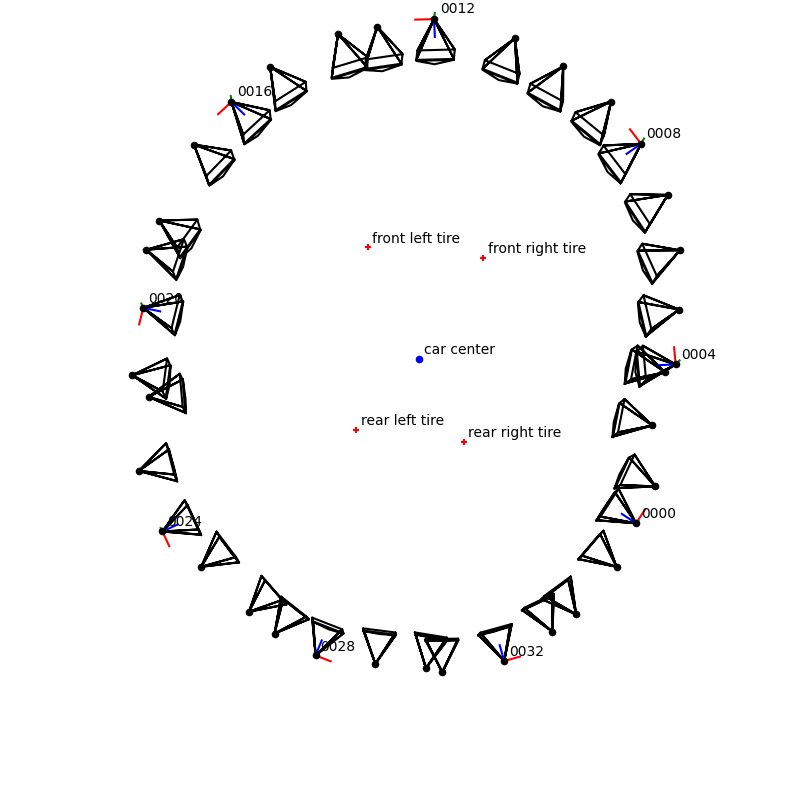
\includegraphics[height=6cm]{images/gaussiansplatting/camera-path-unstabilized.png}
%\caption{\textbf{Original camera path.} Predicted camera poses are unevenly spaced and do not describe a %smooth path around the car. }
%\label{fig:gs-overview}
%\end{figure*}


\begin{center}
  \animategraphics[autoplay,loop, poster=0,width=\linewidth]{5}{images/gaussiansplatting/unstab/img-}{0}{35}
  \label{fig:gs-unstabilized}
  \captionof{figure}{\textbf{Unstabilized camera path} Resulting image merge into a \textit{.gif} animation is too erratic since corresponding camera path has not been stabilized.}
\end{center}


\subsection{$360\degree$ with homography}


\subsection{$360\degree$ with Gaussian Splatting}
\section{Experiments}
\subsection{Rendering at non-training locations}

\subsection{Ablations studies}
\paragraph{Number of views influence}
\paragraph{Depth loss supervision}
\paragraph{View-dependancy effect}
\section{Conclusion}
